\chapter{Theory}

\section{A brief introduction to statistical mechanics}
The discussion in this section is mostly based on the ``Introduction to Computational Chemistry'' textbook written by Jensen~\citep{jensenIntroductionComputationalChemistry2017}, ``Statistical Mechanics: Theory and Molecular Simulation'' by Tuckermann~\citep{tuckermanStatisticalMechanicsTheory2023}, and ``Understanding Molecular Simulation: From Algorithms to Applications'' by Frenkel and Smit~\citep{frenkelUnderstandingMolecularSimulation2002} unless stated otherwise.



\subsection{Partition functions}

\begin{equation}
q = \sum_{i = \text{levels}} g_i e^{-\epsilon_i/kT}
\end{equation}

\begin{equation}
Q = q^N \; \text{(different particles)} \quad Q = \frac{q^N}{N!} \; \text{(identical particles)}
\end{equation}

\begin{equation}
Q = \sum_{i=0}^{\infty} e^{-E_i/kT}
\end{equation}

\begin{equation}
q_{\text{trans}} = \left(\frac{2\pi MkT}{h^2}\right)^{3/2} V
\end{equation}

\begin{equation}
q_{\text{rot}} = \frac{\sqrt{\pi}}{\sigma}\left(\frac{8\pi^2kT}{h^2}\right)^{3/2} \sqrt{I_1I_2I_3}
\end{equation}

\begin{equation}
q_{\text{vib}} = \prod_{i=1}^{3N_{\text{atom}}-6(7)} \frac{e^{-h\nu_i/2kT}}{1-e^{-h\nu_i/kT}}
\end{equation}

\begin{equation}
q_{\text{elec}} = \sum_{i} g_i e^{-\epsilon_i/kT} \approx g_0 e^{-\epsilon_0/kT}
\end{equation}

\begin{align}
\epsilon_{\text{tot}} &= \epsilon_{\text{trans}} + \epsilon_{\text{rot}} + \epsilon_{\text{vib}} + \epsilon_{\text{elec}} \\
q_{\text{tot}} &= q_{\text{trans}} q_{\text{rot}} q_{\text{vib}} q_{\text{elec}} \\
H_{\text{tot}} &= H_{\text{trans}} + H_{\text{rot}} + H_{\text{vib}} + H_{\text{elec}} \\
S_{\text{tot}} &= S_{\text{trans}} + S_{\text{rot}} + S_{\text{vib}} + S_{\text{elec}}
\end{align}

\subsection{Macroscopic properties and thermodynamics functions}

\begin{align}
U &= kT^2 \left(\frac{\partial \ln Q}{\partial T}\right)_V \tag{14.17} \\
A &= -kT\ln Q \tag{14.18}
\end{align}

\begin{align}
P &= -\left(\frac{\partial A}{\partial V}\right)_T = kT\left(\frac{\partial \ln Q}{\partial V}\right)_T \tag{14.19} \\
C_V &= \left(\frac{\partial U}{\partial T}\right)_V = 2kT\left(\frac{\partial \ln Q}{\partial T}\right)_V + kT^2\left(\frac{\partial^2 \ln Q}{\partial T^2}\right)_V \tag{14.20}
\end{align}

\begin{align}
H &= U + PV = kT^2\left(\frac{\partial \ln Q}{\partial T}\right)_V + kTV\left(\frac{\partial \ln Q}{\partial V}\right)_T \tag{14.21} \\
S &= \frac{U-A}{T} = kT\left(\frac{\partial \ln Q}{\partial T}\right)_V + k\ln Q \tag{14.22} \\
G &= H - TS = kTV\left(\frac{\partial \ln Q}{\partial V}\right)_T - kT\ln Q \tag{14.23}
\end{align}

\subsection{Classical forcefields and molecular dynamics}

\subsection{The canonical ensemble}

\subsection{Free energy techniques}

\begin{equation}
V_{\text{G}}(S(x), t) = w \sum_{t' = \tau_{\text{G}}, 2\tau_{\text{G}}, \ldots}^{t' < t} \exp\left(-\frac{(S(x) - s(t'))^2}{2\delta s^2}\right)
\label{eq:biasing_potential}
\end{equation}

\begin{equation}
\label{eq:free_energy_from_metadynamics}
\lim_{t \to \infty} V_G(s,t) \sim -F(s)
\end{equation}

\begin{equation}
V(s, t) = \Delta T \ln\left(1 + \frac{\omega N(s, t)}{\Delta T}\right)
\label{eq:history_dependant_potential}
\end{equation}

\begin{equation}
\label{eq:hill_deposition_rate}
\dot{V}(s,t) = \frac{\omega \Delta T \delta_{s,s(t)}}{\Delta T + \omega N(s,t)} 
= \omega e^{-[V(s,t)/\Delta T]} \delta_{s,s(t)}
\end{equation}

\begin{equation}
w = \omega e^{-[V(s,t)/\Delta T]} \tau_{\text{G}}
\label{eq:hill_height}
\end{equation}

\begin{equation}
\label{eq:free_energy_surface_reconstruction}
\tilde{F}(s,t) = -\frac{T + \Delta T}{\Delta T} V(s,t) 
= -(T + \Delta T) \ln\left(1 + \frac{\omega N(s,t)}{\Delta T} \right)
\end{equation}

\begin{figure}[htbp]
    \centering
    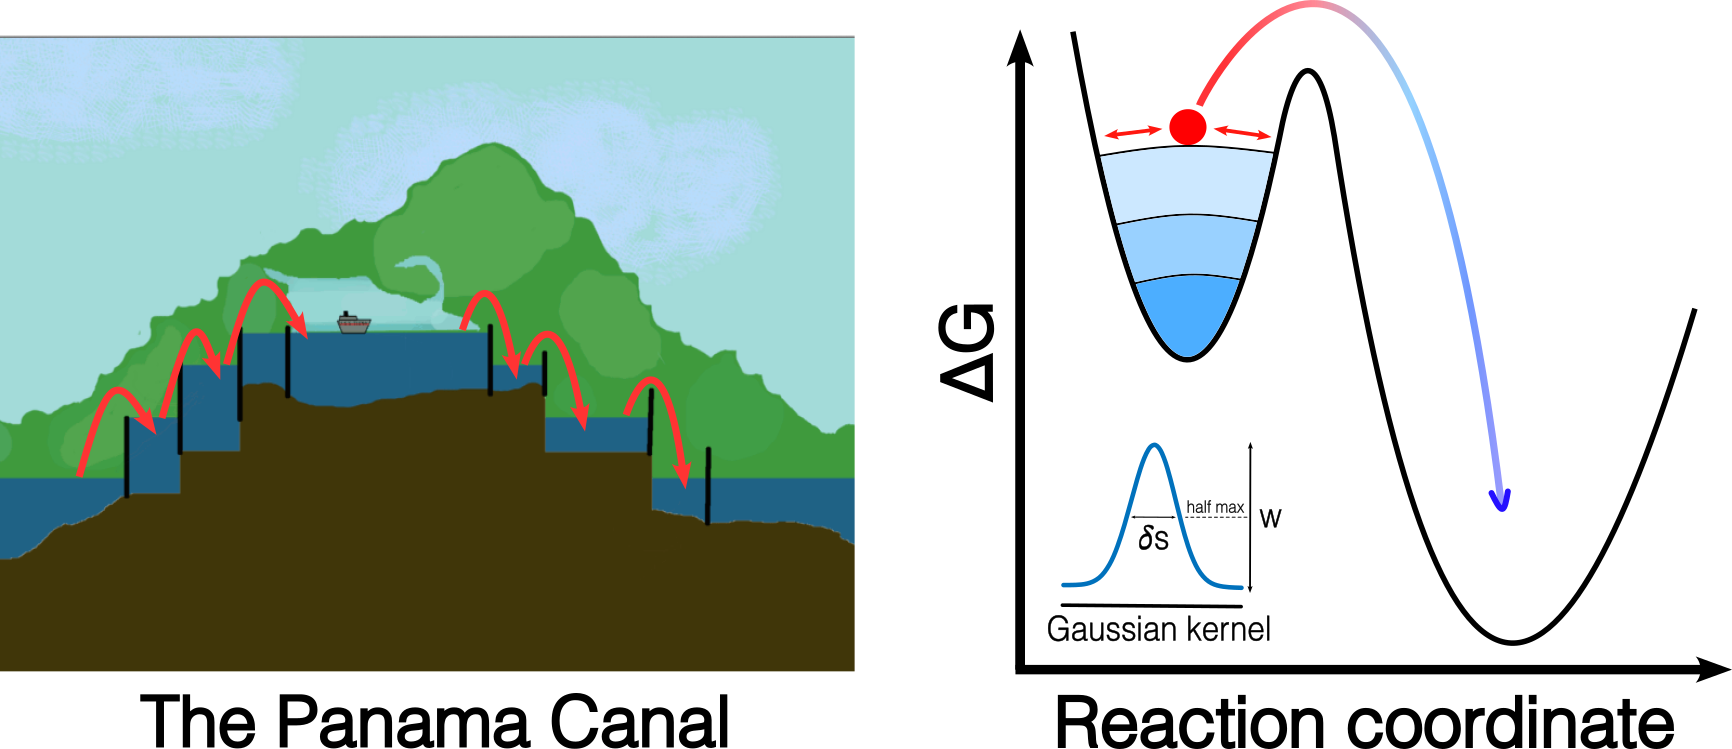
\includegraphics[width=0.8\textwidth]{Figures/2_Theory/theory_metadynamics.png}
    \caption{Metadynamics. The Panama Canal cartoon reproduced from~\citep{HowPanamaCanal}.}
    \label{fig:metadynamics}
\end{figure}



\section{Transition state theory}



\section{Density functional theory}

\subsection{The Kohn-Sham approach}

\subsection{Generalised gradient approximation and PBE functional}

\subsection{\textit{Ab initio} molecular dynamics and GPW method}



\section{Extended tight binding}



\section{Neural network potentials}

\subsection{Deep neural networks}

\subsubsection{Multilayer perceptron}

\subsubsection{Graph neural networks}

\subsubsection{Message passing neural networks}

\subsection{Invariance and equivariance}

\subsection{Behler-Parrinello neural network potentials}

\subsection{Equivariant neural network potentials}